\begin{enumerate}[label=\thesection.\arabic*,ref=\thesection.\theenumi]
\numberwithin{equation}{enumi}
\numberwithin{figure}{enumi}
\numberwithin{table}{enumi}
\item Determine the ratio in which the line $2x+y  - 4=0$ divides the line segment joining the points $\vec{A}(2, - 2)$  and  $\vec{B}(3, 7)$.
\\
\solution
	\iffalse
\documentclass[journal,12pt,twocolumn]{IEEEtran}
\usepackage{graphicx}
\graphicspath{{./chapters/10/7/4/1/figs/}}{}
\usepackage{amsmath,amssymb,amsfonts,amsthm}
\newcommand{\myvec}[1]{\ensuremath{\begin{pmatrix}#1\end{pmatrix}}}
\providecommand{\norm}[1]{\lVert#1\rVert}
\usepackage{listings}
\usepackage{watermark}
\usepackage{titlesec}
\usepackage{caption}
\let\vec\mathbf
\lstset{
frame=single, 
breaklines=true,
columns=fullflexible
}
\thiswatermark{\centering \put(0,-105.0){
\includegraphics[scale=0.15]{/sdcard/IITH/vector/vectpr-4/chapters/10/7/4/1/figs/logo.png}} }
\title{\mytitle}
\title{
Assignment - Vector-4
}
\author{Surajit Sarkar}
\begin{document}
\maketitle
%\tableofcontents
\bigskip
\section{\textbf{Problem}}
Determine the ratio in which the line 2x+y–4=0 divides the line segment joining the points A(2,–2) and B(3,7).
\section{\textbf{Solution}}
\begin{table}[h]
    \centering
    \begin{tabular}{|c|c|}
       \hline
       \textbf{Symbol}&\textbf{Value}  \\
       \hline
	    $\vec{A}$ & $\myvec{2\\-2}$\\
        \hline
	    $\vec{B}$ & $\myvec{3\\7}$\\
        \hline
	    c&$4$\\
        \hline
       $\vec{n}$ & $\myvec{2\\1}$\\
       \hline
    \end{tabular}
    \caption{Parameters}
    \label{tab:my_label}
\end{table}
Given equation
\fi
The given equation can be expressed as
\begin{align}
    \myvec{2&1}\vec{x}&=4\\
\end{align}
Using section formula, the point of division 
\begin{align}
    \vec{P} = \frac{k\vec{B+A}}{k+1}
\end{align}
which upon substitution in the equation of a line yields
\begin{align}
    \implies\vec{n}^{\top}\myvec{\frac{k\vec{B+A}}{k+1}}&=c\\
    \implies k&=\frac{c-\vec{n}^{\top}\vec{A}}{\vec{n}^{\top}\vec{B}-c}\\
\end{align}
upon simplification.  Substituting numerical values, 
\begin{align}
    k=\frac{2}{9}
\end{align}
See Fig. 
\ref{fig:chapters/10/7/4/1vec}.
\begin{figure}[!h]
\centering
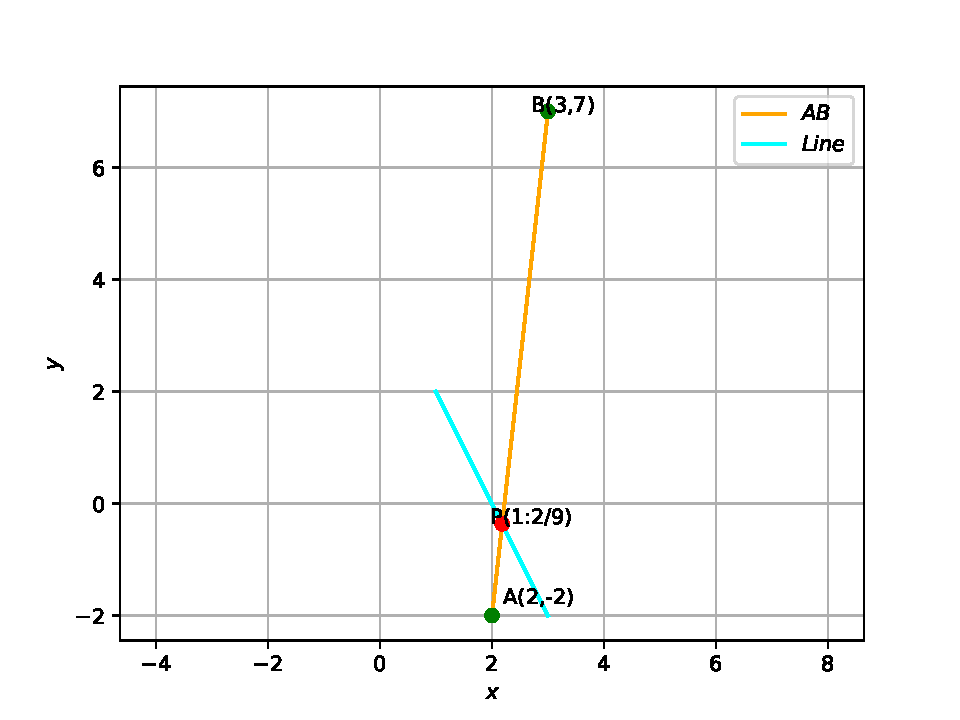
\includegraphics[width=\columnwidth]{chapters/10/7/4/1/figs/vec.pdf}
\caption{}
\label{fig:chapters/10/7/4/1vec}
\end{figure}


\item Find a relation between $x$ and $y$ if the points $(x, y), (1, 2)$  and  $(7, 0)$ are collinear.
\\
\solution
	\iffalse
\documentclass[12pt]{article}
\usepackage{graphicx}
\usepackage{amsmath}
\usepackage{mathtools}
\usepackage{gensymb}

\newcommand{\mydet}[1]{\ensuremath{\begin{vmatrix}#1\end{vmatrix}}}
\providecommand{\brak}[1]{\ensuremath{\left(#1\right)}}
\providecommand{\norm}[1]{\left\lVert#1\right\rVert}
\newcommand{\solution}{\noindent \textbf{Solution: }}
\newcommand{\myvec}[1]{\ensuremath{\begin{pmatrix}#1\end{pmatrix}}}
\let\vec\mathbf

\begin{document}
\begin{center}
\textbf\large{CHAPTER-7 \\ COORDINATE GEOMETRY}
\end{center}
\section*{Excercise 7.4}

Q2. Find a relation between x and y if the points $\vec(x, y), \vec(1, 2) \text{ and } \vec(7, 0)$ are collinear.
\\
\solution
\\
The coordinates are given as
\fi
Let
	\begin{align}
	\vec{A} = \myvec{
		x\\
		y\\
		},
	\vec{B} = \myvec{
		1\\
		2\\
		},
	\vec{C} = \myvec{
		7\\
		0\\
		}
	\end{align}
	Then
	\begin{align}
\vec{D} &=\brak{\vec{A}-\vec{B}} = \brak{\myvec{x \\y } - \myvec{1 \\2 } } = \myvec{x-1 \\ y-2 }\\
\vec{E} &= \brak{\vec{A}-\vec{C}} = \brak{\myvec{x \\ y } - \myvec{7 \\0} } = \myvec{x-7 \\y}
\end{align}
Forming the collinearity matrix
\begin{align}
	\vec{F} &={\myvec{\vec{D}^{\top}\\ \vec{E}^{\top}}}
\end{align}
and performing row reduction,
\begin{align}
\label{eq:chapters/10/7/4/2chem_balance_mat_row}
\myvec{
x-1 & y-2
\\
x-7 & y
}
\xleftrightarrow[]{R_2 = R_2-R_1}
\myvec{
  x-1 & y-2
  \\
	  -6 & 2                 
	  }
	  \\
	\xleftrightarrow[]{R_2 = \frac{R_2}{-6}(x-1)-R_1}
\myvec{
x-1 & y-2
\\
	0 & -\frac{1}{3}(x-1)-(y-2)
}
\end{align}
For the rank of the matrix to be 1,
\begin{align}
	-\frac{1}{3}(x-1)-(y-2)&=0\\
	\implies \myvec{1 & 3}\vec{x} &=7	
\end{align}
For $x=-2, y=3$, see Fig. \ref{fig:chapters/10/7/4/2Fig} verifying that the points are collinear.
\begin{figure}[!h]
	\begin{center} 
	    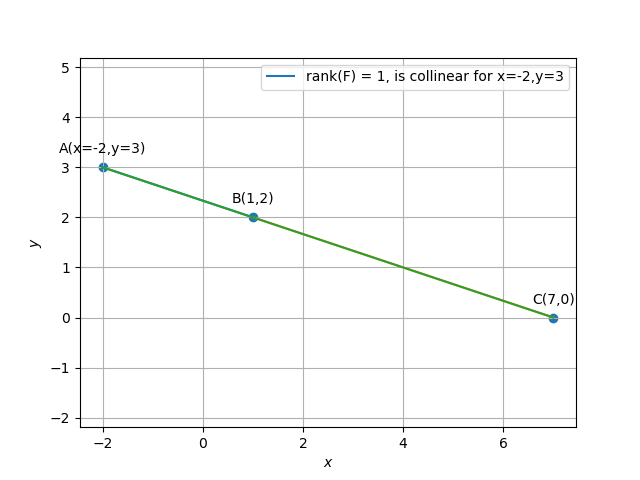
\includegraphics[width=\columnwidth]{chapters/10/7/4/2/figs/sc1.png}
	\end{center}
\caption{}
\label{fig:chapters/10/7/4/2Fig}
\end{figure}



\item The two opposite vertices of a square are $(–1, 2)$  and $ (3, 2)$. Find the coordinates of the other two vertices.
\\
	\iffalse
\documentclass[12pt]{article}
\usepackage{graphicx}
\usepackage{amsmath}
\usepackage{mathtools}
\usepackage{gensymb}

\newcommand{\mydet}[1]{\ensuremath{\begin{vmatrix}#1\end{vmatrix}}}
\providecommand{\brak}[1]{\ensuremath{\left(#1\right)}}
\providecommand{\norm}[1]{\left\lVert#1\right\rVert}
\newcommand{\solution}{\noindent \textbf{Solution: }}
\newcommand{\myvec}[1]{\ensuremath{\begin{pmatrix}#1\end{pmatrix}}}
\let\vec\mathbf

\begin{document}
\begin{center}
\textbf\large{CHAPTER-7 \\ COORDINATE GEOMETRY}

\end{center}
\section*{Excercise 7.4}

Q4.The two opposite vertices of a square are $(–1, 2) \text{ and } (3, 2)$. Find the coordinates of the other two vertices.\\
\fi
\solution
Let
\begin{align}
\vec{A} = \myvec
{
-1 \\
 2\\
},
\vec{C} = 
\myvec
{
3\\
2\\
}
\end{align}

\begin{figure}[!h]
	\begin{center} 
	    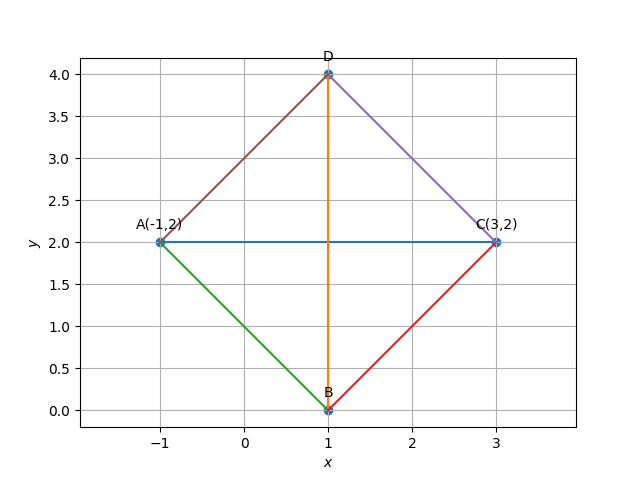
\includegraphics[width=\columnwidth]{chapters/10/7/4/4/figs/square}
	\end{center}
\caption{}
\label{fig:7/4/4/4Fig1}
\end{figure}

Shifting $\vec{A}$ to origin with reference to Fig. \ref{fig:7/4/4/4Fig2},
\begin{align}
\vec{A^{\prime}} =
\myvec{
0 \\
0\\
},
\vec{C^{\prime}} = \vec{C}-\vec{A} = 
\myvec{
4 \\
0\\
}
\end{align}

\begin{figure}[!h]
	\begin{center} 
	    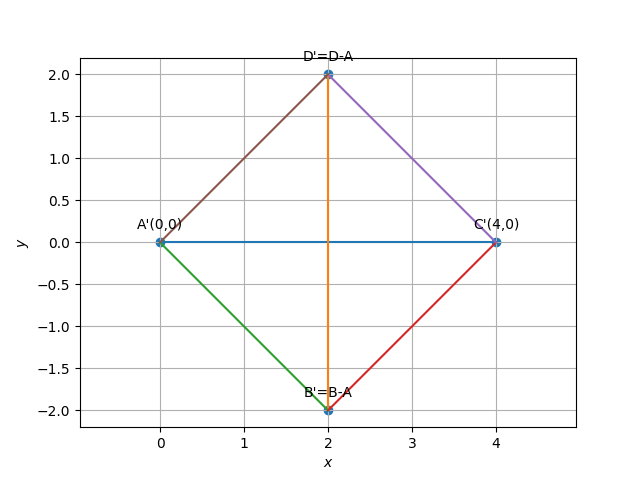
\includegraphics[width=\columnwidth]{chapters/10/7/4/4/figs/square1}
	\end{center}
\caption{}
\label{fig:7/4/4/4Fig2}
\end{figure}
\iffalse
In general,
the angle made by $AC$ with the x-axis is 
		\begin{align}
\beta = \theta + 45\degree
		\end{align}
\fi
Since
\begin{align}
\vec{C} - \vec{A} = \myvec{
4\\
0
} \equiv 
\myvec{
1\\
0
},
	\tan\theta&= \frac{0}{4} \implies 
\theta= 0\degree
\end{align}
		where
$\theta$ is the angle made by $AC$ with the x-axis.
Considering the rotation matrix 
\begin{align}
\vec{P} =
\myvec{
\cos\brak{\frac{\pi}{4}-\theta} & -\sin\brak{\frac{\pi}{4}-\theta} \\
\sin\brak{\frac{\pi}{4}-\theta} & \cos\brak{\frac{\pi}{4}-\theta} 
}
\end{align}
\iffalse
from Fig. \ref{fig:7/4/4/4Fig3},
\begin{align}
\vec{C^{\prime \prime}} = \vec{P}^\top (\vec{C}-\vec{A}) =
\myvec{
\frac{1}{\sqrt{2}} & -\frac{1}{\sqrt{2}} \\
\frac{1}{\sqrt{2}} & \frac{1}{\sqrt{2}}\\
}
\myvec{
4 \\
0\\
} = 
\myvec{
\frac{4}{\sqrt{2}} \\
\frac{4}{\sqrt{2}}\\
}
\end{align}
\begin{align}
\vec{B^{\prime \prime}} = \myvec{
 1&0\\
 0&0\\
}\vec{C^{\prime \prime}}=
\myvec{
 \frac{4}{\sqrt{2}}\\
 0\\
},
\vec{D^{\prime \prime}} = \myvec{
 0&0\\
 0&1\\
}\vec{C^{\prime \prime}}=
\myvec{
 0\\
 \frac{4}{\sqrt{2}}\\
} \text{ and }
\vec{A^{\prime \prime}} =
\myvec{
0 \\
0\\
}
\end{align}
\fi
\begin{figure}[!h]
	\begin{center} 
	    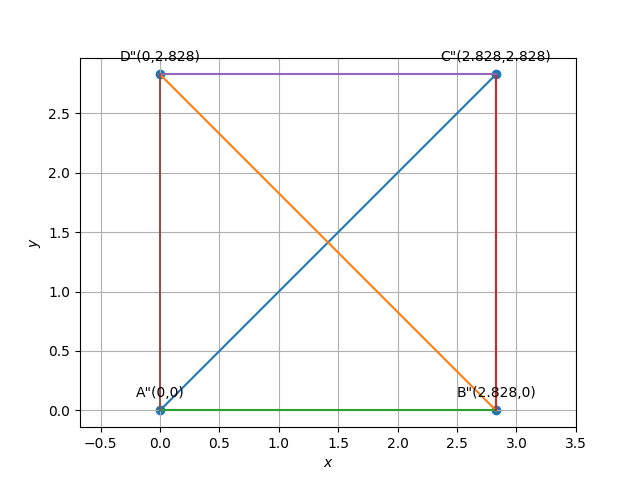
\includegraphics[width=\columnwidth]{chapters/10/7/4/4/figs/square2}
	\end{center}
\caption{}
\label{fig:7/4/4/4Fig3}
\end{figure}

\newpage
\iffalse
Again tranforming(rotating) the coordinates back to the original axis.

We know for anti-clockwise direction the rotation matrix is given as
\begin{align}
\vec{P} =
\myvec{
\cos\theta & -\sin\theta \\
\sin\theta & \cos\theta \\
}
\end{align}

Again we know that the angle is negative so the rotation will be in clockwise direction. So now the transformed(rotated) coordinates $\vec{B} \text{ and } \vec{D}$ are with refrence to 
\fi
from Figure 
%\ref{fig:7/4/4/4Fig4},
\ref{fig:7/4/4/4Fig3},
\begin{align}
	\vec{C^{\prime \prime}} &= \vec{P} (\vec{C}-\vec{A}) 
	\\
\label{eq:7/4/4/4bp}
	\vec{B^{\prime \prime}} &= \myvec{\vec{e}_1 & \vec{0}}\vec{C^{\prime \prime}}
	\\
\label{eq:7/4/4/4dp}
	\vec{D^{\prime \prime}} &= \myvec{ \vec{0} & \vec{e}_2}\vec{C^{\prime \prime}}
\end{align}
Now, 
\begin{align}
\label{eq:7/4/4/4b}
	\vec{B} = \vec{P}^{\top}\vec{B}^{\prime \prime}+\vec{A}
	\\
\label{eq:7/4/4/4d}
	\vec{D} = \vec{P}^{\top}\vec{D}^{\prime \prime}+\vec{A}
\end{align}
by reversing the process of translation and rotation.  Thus, 
from
\eqref{eq:7/4/4/4b}
\eqref{eq:7/4/4/4bp},
\eqref{eq:7/4/4/4d}
and
\eqref{eq:7/4/4/4dp}
\begin{align}
	\vec{B} = \vec{P}^{\top}\myvec{\vec{e}_1 & \vec{0}}\vec{P} (\vec{C}-\vec{A}) +\vec{A}
	\\
	\vec{D} = \vec{P}^{\top}\myvec{\vec{0} & \vec{e}_2  }\vec{P} (\vec{C}-\vec{A}) +\vec{A}
%	\vec{B} &= \brak{(\vec{C}-\vec{A})^{\top}\vec{P}^{\top} \vec{e}_1}\vec{P}^{\top}\vec{e}_1+\vec{A}
%	\\
%	\vec{D} &= \brak{(\vec{C}-\vec{A})^{\top}\vec{P}^{\top} \vec{e}_2}\vec{P}^{\top}\vec{e}_2+\vec{A}
\end{align}
yielding
		\begin{align}
\vec{B}=
\myvec{
1\\
0
},
\vec{D}
\myvec{
1\\
4
}.
		\end{align}
\iffalse
\begin{align}
\vec{B^{\prime}} &= \vec{P}\vec{B^{\prime \prime}} = \myvec{
\frac{1}{\sqrt{2}} & \frac{1}{\sqrt{2}} \\
-\frac{1}{\sqrt{2}} & \frac{1}{\sqrt{2}}\\
}
\myvec{
 \frac{4}{\sqrt{2}}\\
 0\\
} = 
\myvec{
2 \\
-2\\
}\\
\vec{D^{\prime}} &= \vec{P}\vec{D^{\prime \prime}} = \myvec{
\frac{1}{\sqrt{2}} & \frac{1}{\sqrt{2}} \\
-\frac{1}{\sqrt{2}} & \frac{1}{\sqrt{2}}\\
}
\myvec{
 0\\
 \frac{4}{\sqrt{2}}\\
} = 
\myvec{
2 \\
2 \\
}
\end{align}

\begin{figure}[!h]
	\begin{center} 
	    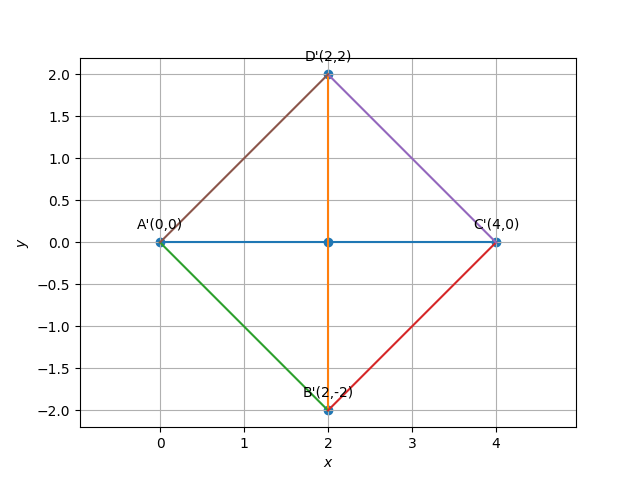
\includegraphics[width=\columnwidth]{chapters/10/7/4/4/figs/square3}
	\end{center}
\caption{}
\label{fig:7/4/4/4Fig4}
\end{figure}

Again transforming(shifting) the axis back to the original with refrence to Figure \ref{fig:7/4/4/4Fig5}
\begin{align}
\vec{B} &= \vec{B^{\prime}}+\vec{A} = \myvec{
2 \\
-2\\
}+\myvec{
-1 \\
2\\
} = 
\myvec{
1 \\
0\\
}\\
\vec{D} &= \vec{D^{\prime}}+\vec{A} = \myvec{
2 \\
2\\
}+\myvec{
-1 \\
2\\
} = 
\myvec{
1 \\
4 \\
}
\end{align}

Hence, the other two vertices are $\vec{B}(1,0) \text{ and } \vec{D}(1,4)$   

\begin{figure}[!h]
	\begin{center} 
	    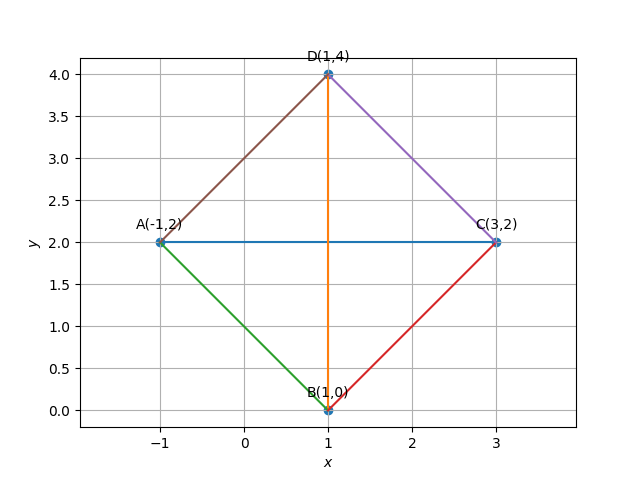
\includegraphics[width=\columnwidth]{chapters/10/7/4/4/figs/square4}
	\end{center}
\caption{}
\label{fig:7/4/4/4Fig5}
\end{figure}
which can also be expressed as
\begin{align}
\vec{B} &= \vec{A} + \vec{P}\myvec{
\vec{e_{1}}&\vec{0}\\
}
\vec{P}^\top \brak{\vec{C}-\vec{A}}\\
\vec{D} &= \vec{A} + \vec{P}\myvec{
\vec{0}&\vec{e_{2}}\\
}
\vec{P}^\top \brak{\vec{C}-\vec{A}}\\
\end{align}
where $\vec{P}$ is the rotation matrix and $\vec{A} \text{ and } \vec{C}$ are the position vectors of opposite vertices.

Derivation of the above formulas:

We know that after shifting the axis and rotating by the required angle any arbitrary square will be aligned with the x and y axis so that we can directly get the vectors $\vec{B} \text{ and } \vec{D}$ as follows
\begin{align}
\vec{C^{\prime\prime}} &= \vec{P}^\top \brak{\vec{C} - \vec{A}}\\
\vec{B^{\prime\prime}} &= \myvec{
\vec{e_{1}} & \vec{0}
}\vec{C^{\prime\prime}} = \myvec{
\vec{e_{1}} & \vec{0}
}\vec{P}^\top \brak{\vec{C} - \vec{A}}\\
\vec{B^{\prime}} &= \vec{P} \vec{B^{\prime\prime}}  = \vec{P}\myvec{
\vec{e_{1}} & \vec{0}
}\vec{P}^\top \brak{\vec{C} - \vec{A}}\\
\vec{B} &= \vec{A}+\vec{B^{\prime}}\\
 &= \vec{A} + \vec{P}\myvec{
\vec{e_{1}}&\vec{0}\\
}
\vec{P}^\top\brak{\vec{C}-\vec{A}}
\end{align}

Similarly for D it can be derived as
\begin{align}
\vec{C^{\prime\prime}} &= \vec{P}^\top \brak{\vec{C} - \vec{A}}\\
\vec{D^{\prime\prime}} &= \myvec{
\vec{0} & \vec{e_{2}}
}\vec{C^{\prime\prime}} = \myvec{
\vec{0} & \vec{e_{2}}
}\vec{P}^\top \brak{\vec{C} - \vec{A}}\\
\vec{D^{\prime}} &= \vec{P} \vec{D^{\prime\prime}} = \vec{P} \myvec{
\vec{0} & \vec{e_{2}}
}\vec{P}^\top \brak{\vec{C} - \vec{A}}\\
\vec{D} &= \vec{A}+\vec{D^{\prime}}\\
 &= \vec{A} + \vec{P}\myvec{
\vec{0}&\vec{e_{2}}\\
}
\vec{P}^\top\brak{\vec{C}-\vec{A}}
\end{align}


Verification of the above formula for the given question

\begin{align}
\vec{B} &= \myvec{
-1\\
2\\
}+\myvec{
\frac{1}{\sqrt{2}} & \frac{1}{\sqrt{2}} \\
-\frac{1}{\sqrt{2}} & \frac{1}{\sqrt{2}}\\
}\myvec{
 1&0\\
 0&0\\
}\myvec{
\frac{1}{\sqrt{2}} & -\frac{1}{\sqrt{2}} \\
\frac{1}{\sqrt{2}} & \frac{1}{\sqrt{2}}\\
}\myvec{
4\\
0\\
}\\
 &= \myvec{
-1\\
2\\
}+\myvec{
\frac{1}{\sqrt{2}} & \frac{1}{\sqrt{2}} \\
-\frac{1}{\sqrt{2}} & \frac{1}{\sqrt{2}}\\
}\myvec{
 1&0\\
 0&0\\
}\myvec{
\frac{4}{\sqrt{2}}\\
\frac{4}{\sqrt{2}}\\
}\\
 &= \myvec{
-1\\
2\\
}+\myvec{
\frac{1}{\sqrt{2}} & \frac{1}{\sqrt{2}} \\
-\frac{1}{\sqrt{2}} & \frac{1}{\sqrt{2}}\\
}\myvec{
\frac{4}{\sqrt{2}}\\
0\\
}\\
 &= \myvec{
-1\\
2\\
}+\myvec{
2\\
-2\\
}\\
 &= \myvec{
1\\
0\\
}\\
\vec{D} &= \myvec{
-1\\
2\\
}+\myvec{
\frac{1}{\sqrt{2}} & \frac{1}{\sqrt{2}} \\
-\frac{1}{\sqrt{2}} & \frac{1}{\sqrt{2}}\\
}\myvec{
 0&0\\
 0&1\\
}\myvec{
\frac{1}{\sqrt{2}} & -\frac{1}{\sqrt{2}} \\
\frac{1}{\sqrt{2}} & \frac{1}{\sqrt{2}}\\
}\myvec{
4\\
0\\
}\\
 &= \myvec{
-1\\
2\\
}+\myvec{
\frac{1}{\sqrt{2}} & \frac{1}{\sqrt{2}} \\
-\frac{1}{\sqrt{2}} & \frac{1}{\sqrt{2}}\\
}\myvec{
 0&0\\
 0&1\\
}\myvec{
\frac{4}{\sqrt{2}}\\
\frac{4}{\sqrt{2}}\\
}\\
 &= \myvec{
-1\\
2\\
}+\myvec{
\frac{1}{\sqrt{2}} & \frac{1}{\sqrt{2}} \\
-\frac{1}{\sqrt{2}} & \frac{1}{\sqrt{2}}\\
}\myvec{
0\\
\frac{4}{\sqrt{2}}\\
}\\
 &= \myvec{
-1\\
2\\
}+\myvec{
2\\
2\\
}\\
 &= \myvec{
1\\
4\\
}
\end{align}
\fi








\item The vertices of a $\triangle ABC$ are $\vec{A}(4,6), \vec{B}(1,5)$ and  $\vec{C}(7,2)$. A line is drawn to intersect sides $AB$ and $AC$ at $\vec{D}$ and $\vec{E}$ respectively, such that $\frac{AD}{AB} = \frac{AE}{AC} = \frac{1}{4}$. Calculate the area of $\triangle ADE$ and compare it with the area of the $\triangle ABC$.
\\
\solution
	\iffalse
\documentclass[12pt]{article}
\usepackage{graphicx}
%\documentclass[journal,12pt,twocolumn]{IEEEtran}
\usepackage[none]{hyphenat}
\usepackage{graphicx}
\usepackage{listings}
\usepackage[english]{babel}
\usepackage{graphicx}
\usepackage{caption}
\usepackage[parfill]{parskip}
\usepackage{hyperref}
\usepackage{booktabs}
%\usepackage{setspace}\doublespacing\pagestyle{plain}
\def\inputGnumericable{}
\usepackage{color}                                            %%
    \usepackage{array}                                            %%
    \usepackage{longtable}                                        %%
    \usepackage{calc}                                             %%
    \usepackage{multirow}                                         %%
    \usepackage{hhline}                                           %%
    \usepackage{ifthen}
\usepackage{array}
\usepackage{amsmath}   % for having text in math mode
\usepackage{parallel,enumitem}
\usepackage{listings}
\lstset{
language=tex,
frame=single, 
breaklines=true
}
  
%Following 2 lines were added to remove the blank page at the beginning
\usepackage{atbegshi}% http://ctan.org/pkg/atbegshi
\AtBeginDocument{\AtBeginShipoutNext{\AtBeginShipoutDiscard}}
%
%New macro definitions
\newcommand{\mydet}[1]{\ensuremath{\begin{vmatrix}#1\end{vmatrix}}}
\providecommand{\brak}[1]{\ensuremath{\left(#1\right)}}
\providecommand{\norm}[1]{\left\lVert#1\right\rVert}
\newcommand{\solution}{\noindent \textbf{Solution: }}
\newcommand{\myvec}[1]{\ensuremath{\begin{pmatrix}#1\end{pmatrix}}}
\let\vec\mathbf
\begin{document}
\begin{center}
\title{\textbf{Coordinate Geometry}}
\date{\vspace{-5ex}} %Not to print date automatically
\maketitle
\end{center}
\setcounter{page}{1}
\section*{10$^{th}$ Maths - Chapter 7}
This is Problem-6 from Exercise 7.4
\begin{enumerate}
\item The vertices of $\triangle ABC$ are $\myvec{4 \\ 6}, \myvec{1\\5}, \myvec{7\\2}$. A line is drawn to intersect sides AB and AC at D and E respectively, such that $\dfrac{AD}{AB}=\dfrac{AE}{AC}=\dfrac{1}{4}$. Calculate the area of the $\triangle ADE$ and compare it with the area of $\triangle ABC$.\\
\solution 
\fi
		The input parameters for this problem are available in Table \eqref{table:chapters/10/7/4/61}.
\begin{table}[ht!]\centering
%%%%%%%%%%%%%%%%%%%%%%%%%%%%%%%%%%%%%%%%%%%%%%%%%%%%%%%%%%%%%%%%%%%%%%
%%                                                                  %%
%%  This is the header of a LaTeX2e file exported from Gnumeric.    %%
%%                                                                  %%
%%  This file can be compiled as it stands or included in another   %%
%%  LaTeX document. The table is based on the longtable package so  %%
%%  the longtable options (headers, footers...) can be set in the   %%
%%  preamble section below (see PRAMBLE).                           %%
%%                                                                  %%
%%  To include the file in another, the following two lines must be %%
%%  in the including file:                                          %%
%%        \def\inputGnumericTable{}                                 %%
%%  at the beginning of the file and:                               %%
%%        \input{name-of-this-file.tex}                             %%
%%  where the table is to be placed. Note also that the including   %%
%%  file must use the following packages for the table to be        %%
%%  rendered correctly:                                             %%
%%    \usepackage[latin1]{inputenc}                                 %%
%%    \usepackage{color}                                            %%
%%    \usepackage{array}                                            %%
%%    \usepackage{longtable}                                        %%
%%    \usepackage{calc}                                             %%
%%    \usepackage{multirow}                                         %%
%%    \usepackage{hhline}                                           %%
%%    \usepackage{ifthen}                                           %%
%%  optionally (for landscape tables embedded in another document): %%
%%    \usepackage{lscape}                                           %%
%%                                                                  %%
%%%%%%%%%%%%%%%%%%%%%%%%%%%%%%%%%%%%%%%%%%%%%%%%%%%%%%%%%%%%%%%%%%%%%%



%%  This section checks if we are begin input into another file or  %%
%%  the file will be compiled alone. First use a macro taken from   %%
%%  the TeXbook ex 7.7 (suggestion of Han-Wen Nienhuys).            %%
\def\ifundefined#1{\expandafter\ifx\csname#1\endcsname\relax}


%%  Check for the \def token for inputed files. If it is not        %%
%%  defined, the file will be processed as a standalone and the     %%
%%  preamble will be used.                                          %%
\ifundefined{inputGnumericTable}

%%  We must be able to close or not the document at the end.        %%
	\def\gnumericTableEnd{\end{document}}


%%%%%%%%%%%%%%%%%%%%%%%%%%%%%%%%%%%%%%%%%%%%%%%%%%%%%%%%%%%%%%%%%%%%%%
%%                                                                  %%
%%  This is the PREAMBLE. Change these values to get the right      %%
%%  paper size and other niceties.                                  %%
%%                                                                  %%
%%%%%%%%%%%%%%%%%%%%%%%%%%%%%%%%%%%%%%%%%%%%%%%%%%%%%%%%%%%%%%%%%%%%%%

	\documentclass[12pt%
			  %,landscape%
                    ]{report}
       \usepackage[latin1]{inputenc}
       \usepackage{fullpage}
       \usepackage{color}
       \usepackage{array}
       \usepackage{longtable}
       \usepackage{calc}
       \usepackage{multirow}
       \usepackage{hhline}
       \usepackage{ifthen}

	\begin{document}


%%  End of the preamble for the standalone. The next section is for %%
%%  documents which are included into other LaTeX2e files.          %%
\else

%%  We are not a stand alone document. For a regular table, we will %%
%%  have no preamble and only define the closing to mean nothing.   %%
    \def\gnumericTableEnd{}

%%  If we want landscape mode in an embedded document, comment out  %%
%%  the line above and uncomment the two below. The table will      %%
%%  begin on a new page and run in landscape mode.                  %%
%       \def\gnumericTableEnd{\end{landscape}}
%       \begin{landscape}


%%  End of the else clause for this file being \input.              %%
\fi

%%%%%%%%%%%%%%%%%%%%%%%%%%%%%%%%%%%%%%%%%%%%%%%%%%%%%%%%%%%%%%%%%%%%%%
%%                                                                  %%
%%  The rest is the gnumeric table, except for the closing          %%
%%  statement. Changes below will alter the table's appearance.     %%
%%                                                                  %%
%%%%%%%%%%%%%%%%%%%%%%%%%%%%%%%%%%%%%%%%%%%%%%%%%%%%%%%%%%%%%%%%%%%%%%

\providecommand{\gnumericmathit}[1]{#1} 
%%  Uncomment the next line if you would like your numbers to be in %%
%%  italics if they are italizised in the gnumeric table.           %%
%\renewcommand{\gnumericmathit}[1]{\mathit{#1}}
\providecommand{\gnumericPB}[1]%
{\let\gnumericTemp=\\#1\let\\=\gnumericTemp\hspace{0pt}}
 \ifundefined{gnumericTableWidthDefined}
        \newlength{\gnumericTableWidth}
        \newlength{\gnumericTableWidthComplete}
        \newlength{\gnumericMultiRowLength}
        \global\def\gnumericTableWidthDefined{}
 \fi
%% The following setting protects this code from babel shorthands.  %%
 \ifthenelse{\isundefined{\languageshorthands}}{}{\languageshorthands{english}}
%%  The default table format retains the relative column widths of  %%
%%  gnumeric. They can easily be changed to c, r or l. In that case %%
%%  you may want to comment out the next line and uncomment the one %%
%%  thereafter                                                      %%
\providecommand\gnumbox{\makebox[0pt]}
%%\providecommand\gnumbox[1][]{\makebox}

%% to adjust positions in multirow situations                       %%
\setlength{\bigstrutjot}{\jot}
\setlength{\extrarowheight}{\doublerulesep}

%%  The \setlongtables command keeps column widths the same across  %%
%%  pages. Simply comment out next line for varying column widths.  %%
\setlongtables

\setlength\gnumericTableWidth{%
	53pt+%
	53pt+%
	82pt+%
	53pt+%
0pt}
\def\gumericNumCols{4}
\setlength\gnumericTableWidthComplete{\gnumericTableWidth+%
         \tabcolsep*\gumericNumCols*2+\arrayrulewidth*\gumericNumCols}
\ifthenelse{\lengthtest{\gnumericTableWidthComplete > \linewidth}}%
         {\def\gnumericScale{1*\ratio{\linewidth-%
                        \tabcolsep*\gumericNumCols*2-%
                        \arrayrulewidth*\gumericNumCols}%
{\gnumericTableWidth}}}%
{\def\gnumericScale{1}}

%%%%%%%%%%%%%%%%%%%%%%%%%%%%%%%%%%%%%%%%%%%%%%%%%%%%%%%%%%%%%%%%%%%%%%
%%                                                                  %%
%% The following are the widths of the various columns. We are      %%
%% defining them here because then they are easier to change.       %%
%% Depending on the cell formats we may use them more than once.    %%
%%                                                                  %%
%%%%%%%%%%%%%%%%%%%%%%%%%%%%%%%%%%%%%%%%%%%%%%%%%%%%%%%%%%%%%%%%%%%%%%

\ifthenelse{\isundefined{\gnumericColA}}{\newlength{\gnumericColA}}{}\settowidth{\gnumericColA}{\begin{tabular}{@{}p{53pt*\gnumericScale}@{}}x\end{tabular}}
\ifthenelse{\isundefined{\gnumericColB}}{\newlength{\gnumericColB}}{}\settowidth{\gnumericColB}{\begin{tabular}{@{}p{53pt*\gnumericScale}@{}}x\end{tabular}}
\ifthenelse{\isundefined{\gnumericColC}}{\newlength{\gnumericColC}}{}\settowidth{\gnumericColC}{\begin{tabular}{@{}p{82pt*\gnumericScale}@{}}x\end{tabular}}
\ifthenelse{\isundefined{\gnumericColD}}{\newlength{\gnumericColD}}{}\settowidth{\gnumericColD}{\begin{tabular}{@{}p{53pt*\gnumericScale}@{}}x\end{tabular}}

	\begin{center}
\begin{tabular}[c]{%
	b{\gnumericColA}%
	b{\gnumericColB}%
	b{\gnumericColC}%
	b{\gnumericColD}%
	}

%%%%%%%%%%%%%%%%%%%%%%%%%%%%%%%%%%%%%%%%%%%%%%%%%%%%%%%%%%%%%%%%%%%%%%
%%  The longtable options. (Caption, headers... see Goosens, p.124) %%
%	\caption{The Table Caption.}             \\	%
% \hline	% Across the top of the table.
%%  The rest of these options are table rows which are placed on    %%
%%  the first, last or every page. Use \multicolumn if you want.    %%

%%  Header for the first page.                                      %%
%	\multicolumn{4}{c}{The First Header} \\ \hline 
%	\multicolumn{1}{c}{colTag}	%Column 1
%	&\multicolumn{1}{c}{colTag}	%Column 2
%	&\multicolumn{1}{c}{colTag}	%Column 3
%	&\multicolumn{1}{c}{colTag}	\\ \hline %Last column
%	\endfirsthead

%%  The running header definition.                                  %%
%	\hline
%	\multicolumn{4}{l}{\ldots\small\slshape continued} \\ \hline
%	\multicolumn{1}{c}{colTag}	%Column 1
%	&\multicolumn{1}{c}{colTag}	%Column 2
%	&\multicolumn{1}{c}{colTag}	%Column 3
%	&\multicolumn{1}{c}{colTag}	\\ \hline %Last column
%	\endhead

%%  The running footer definition.                                  %%
%	\hline
%	\multicolumn{4}{r}{\small\slshape continued\ldots} \\
%	\endfoot

%%  The ending footer definition.                                   %%
%	\multicolumn{4}{c}{That's all folks} \\ \hline 
%	\endlastfoot
%%%%%%%%%%%%%%%%%%%%%%%%%%%%%%%%%%%%%%%%%%%%%%%%%%%%%%%%%%%%%%%%%%%%%%

\hhline{|-|-|-~}
	 \multicolumn{1}{|p{\gnumericColA}|}%
	{\gnumericPB{\centering}\gnumbox{\textbf{Symbol}}}
	&\multicolumn{1}{p{\gnumericColB}|}%
	{\gnumericPB{\centering}\gnumbox{\textbf{Value}}}
	&\multicolumn{1}{p{\gnumericColC}|}%
	{\gnumericPB{\centering}\gnumbox{\textbf{Description}}}
	&
\\
\hhline{|---|~}
	 \multicolumn{1}{|p{\gnumericColA}|}%
	{\gnumericPB{\centering}\gnumbox{$\vec{A}$}}
	&\multicolumn{1}{p{\gnumericColB}|}%
	{\gnumericPB{\centering}\gnumbox{$\myvec{4\\6}$}}
	&\multicolumn{1}{p{\gnumericColC}|}%
	{\gnumericPB{\centering}\gnumbox{First point}}
	&
\\
\hhline{|---|~}
	 \multicolumn{1}{|p{\gnumericColA}|}%
	{\gnumericPB{\centering}\gnumbox{$\vec{B}$}}
	&\multicolumn{1}{p{\gnumericColB}|}%
	{\gnumericPB{\centering}\gnumbox{$\myvec{1\\5}$}}
	&\multicolumn{1}{p{\gnumericColC}|}%
	{\gnumericPB{\centering}\gnumbox{Second point}}
	&
\\

\hhline{|---|~}
	 \multicolumn{1}{|p{\gnumericColA}|}%
	{\gnumericPB{\centering}\gnumbox{$\vec{C}$}}
	&\multicolumn{1}{p{\gnumericColB}|}%
	{\gnumericPB{\centering}\gnumbox{$\myvec{7\\2}$}}
	&\multicolumn{1}{p{\gnumericColC}|}%
	{\gnumericPB{\centering}\gnumbox{Third point}}
	&
\\

\hhline{|---|~}
	 \multicolumn{1}{|p{\gnumericColA}|}%
	{\gnumericPB{\centering}\gnumbox{$\vec{D}$}}
	&\multicolumn{1}{p{\gnumericColB}|}%
	{\gnumericPB{\centering}\gnumbox{$?$}}
	&\multicolumn{1}{p{\gnumericColC}|}%
	{\gnumericPB{\centering}\gnumbox{Desired point}}
	&
\\
\hhline{|---|~}
	 \multicolumn{1}{|p{\gnumericColA}|}%
	{\gnumericPB{\centering}\gnumbox{$\vec{E}$}}
	&\multicolumn{1}{p{\gnumericColB}|}%
	{\gnumericPB{\centering}\gnumbox{$?$}}
	&\multicolumn{1}{p{\gnumericColC}|}%
	{\gnumericPB{\centering}\gnumbox{Desired point}}
	&
\\

\hhline{|-|-|-|~}
\end{tabular}
	\end{center}

\ifthenelse{\isundefined{\languageshorthands}}{}{\languageshorthands{\languagename}}
\gnumericTableEnd
\caption{}
\label{table:chapters/10/7/4/61}	
\end{table}
%
Given,
\begin{align}
\frac{AD}{AB}=\frac{AE}{AC}=\frac{1}{4}\label{eq:chapters/10/7/4/61}
\end{align}
\iffalse
From \eqref{eq:chapters/10/7/4/61},
\begin{align}
\frac{AD}{AB} &=\frac{1}{4}\\
\frac{AD}{BD} &=\frac{1}{3}
\end{align}
$\vec{D}$ divides $\vec{A}\vec{B}$ in the ratio of 
\fi
	Using Section formula,
\begin{align}
\vec{D} &=\frac{\vec{A}+n\vec{B}}{1+n}\label{eq:chapters/10/7/4/64}
\\
	&=\myvec{\frac{13}{4}\\[2pt] \frac{23}{4}}
\end{align}
substituting
		$n = \frac{1}{3}$.
%part-2
Similarly,
\iffalse
From \eqref{eq:chapters/10/7/4/61},
\begin{align}
\frac{AE}{AC} &=\frac{1}{4}\\
\frac{AE}{CE} &=\frac{1}{3}
\end{align}
Point $\vec{E}$ divides $\vec{A}\vec{C}$ in the ratio of $n = \frac{1}{3}$.
Using Section formula,
\fi
\begin{align}
\vec{E} &=\frac{\vec{A}+n\vec{C}}{1+n}\label{eq:chapters/10/7/4/611}
	&=\myvec{\frac{19}{4}\\[2pt] \frac{20}{4}}
\end{align}
and
\begin{align}
	\vec{A}- \vec{D} &= \myvec{4\\6}-\myvec{\frac{13}{4}\\[2pt] \frac{23}{4}}=\myvec{\frac{3}{4}\\[2pt] \frac{1}{4}}\label{eq:chapters/10/7/4/617}\\
	  \vec{A}- \vec{E} &= \myvec{4\\6}-\myvec{\frac{19}{4}\\[2pt] \frac{20}{4}}=\myvec{\frac{-3}{4}\\[2pt]1}\label{eq:chapters/10/7/4/618}
\end{align}
yielding
\begin{align}
	ar(ABD) &=\frac{1}{2} \norm{\brak{\vec{A}-\vec{D}}  \times 
   \brak{\vec{A}- \vec{E}}} \label{eq:chapters/10/7/4/616} \\
	&=\frac{1}{2}\mydet{\frac{3}{4} & \frac{-3}{4}\\[2pt] \frac{1}{4} & 1}  
	\\
	&=	\frac{15}{32}
\end{align}
Similarly,
\begin{align}
	\vec{A}- \vec{B} &= \myvec{4\\6}-\myvec{1\\5}=\myvec{3\\1}\label{eq:chapters/10/7/4/621}\\
	  \vec{B}-\vec{C} &= \myvec{1\\5}-\myvec{7\\2}=\myvec{-6\\3}\label{eq:chapters/10/7/4/622}
\end{align}
yielding
  \begin{align}
	  ar(ABC) &=\frac{1}{2} \norm{\brak{\vec{A}-\vec{B}}  \times 
   \brak{\vec{B}- \vec{C}}} \label{eq:chapters/10/7/4/620} \\
	  &=\frac{1}{2}\mydet{3 & -6\\1 & 3}  
	  \\
	&=	\frac{15}{2}
\end{align}
Thus,
\begin{align}
	\frac{ar\brak{ADE}}{ar\brak{ABC}}=\frac{1}{16}
\end{align}
See Fig. 
\ref{fig:chapters/10/7/4/6Fig1}.
\begin{figure}[!h]
 \begin{center}
 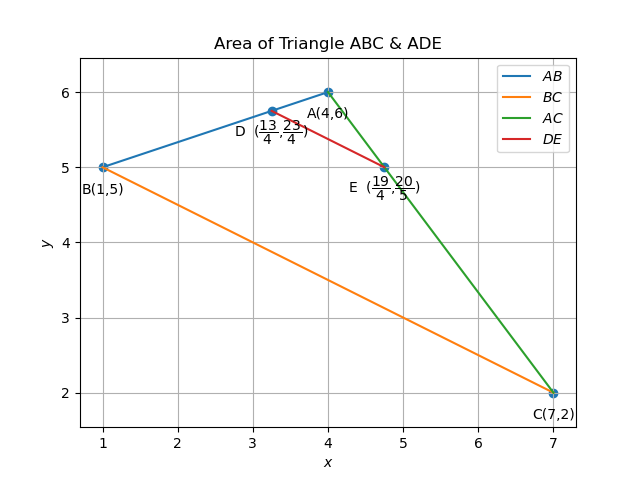
\includegraphics[width=\columnwidth]{chapters/10/7/4/6/figs/fig.png}
 \end{center}
\caption{}
\label{fig:chapters/10/7/4/6Fig1}
\end{figure}

\item Let $\vec{A}(4, 2), \vec{B}(6, 5)$  and $ \vec{C}(1, 4)$ be the vertices of $\triangle ABC$.

\begin{enumerate}
\item The median from $\vec{A}$ meets $BC$ at $\vec{D}$. Find the coordinates of the point $\vec{D}$.
\item Find the coordinates of the point $\vec{P}$ on $AD$ such that $AP : PD = 2 : 1$.
\item Find the coordinates of points $\vec{Q}$ and $\vec{R}$ on medians $BE$ and $CF$ respectively such that $BQ : QE = 2 : 1$  and  $CR : RF = 2 : 1$.
\item What do you observe?
\item If $\vec{A}, \vec{B}$ and $\vec{C}$  are the vertices of $\triangle ABC$, find the coordinates of the centroid of the triangle.
\end{enumerate}
\solution
	\iffalse
\documentclass[12pt]{article}
\usepackage{graphicx}
\usepackage[none]{hyphenat}
\usepackage{graphicx}
\usepackage{listings}
\usepackage[english]{babel}
\usepackage{graphicx}
\usepackage{caption} 
\usepackage{booktabs}
\usepackage{array}
\usepackage{amssymb} % for \because
\usepackage{amsmath}   % for having text in math mode
\usepackage{extarrows} % for Row operations arrows
\usepackage{listings}
\usepackage[utf8]{inputenc}
\lstset{
  frame=single,
  breaklines=true
}
\usepackage{hyperref}
  
%Following 2 lines were added to remove the blank page at the beginning
\usepackage{atbegshi}% http://ctan.org/pkg/atbegshi
\AtBeginDocument{\AtBeginShipoutNext{\AtBeginShipoutDiscard}}


%New macro definitions
\newcommand{\mydet}[1]{\ensuremath{\begin{vmatrix}#1\end{vmatrix}}}
\providecommand{\brak}[1]{\ensuremath{\left(#1\right)}}
\newcommand{\solution}{\noindent \textbf{Solution: }}
\newcommand{\myvec}[1]{\ensuremath{\begin{pmatrix}#1\end{pmatrix}}}
\providecommand{\norm}[1]{\left\lVert#1\right\rVert}
\providecommand{\abs}[1]{\left\vert#1\right\vert}
\let\vec\mathbf

\begin{document}

\begin{center}
\title{\textbf{VECTORS}}
\date{\vspace{-5ex}} %Not to print date automatically
\maketitle
\end{center}

\section{10$^{th}$ Maths - EXERCISE-7.4}

Let A(4, 2), B(6, 5) and C(1, 4) be the vertices of $\triangle ABC$
\begin{enumerate}
\item The median from A meets BC at D. Find the coordinates of the point D.
\item Find the coordinates of the point P on AD such that $AP : PD = 2 : 1$
\item Find the coordinates of points Q and R on medians BE and CF respectively such
that $BQ : QE = 2 : 1 \text{and} CR : RF = 2 : 1.$
\item What do yo observe?
\item If $A(x_1, y_1), B(x_2, y_2) \text{and} C(x_3, y_3)$ are the vertices of $\triangle ABC$, find the coordinates of the centroid of the triangle.
\end{enumerate}

Given points are
\begin{align}
\vec{A}=\myvec{4\\ 2} ,
\vec{B}=\myvec{6\\ 5} ,
\vec{C}=\myvec{1\\ 4}
\end{align}
\fi

\begin{enumerate}
\item 
\begin{align}
\vec{D}&=\frac{\vec{B}+\vec{C}}{2}\\
&=\myvec{\frac{7}{2}\\[2pt] \frac{9}{2}}\\
\vec{E}&=\frac{\vec{A}+\vec{C}}{2}\\
&=\myvec{\frac{5}{2}\\ 3}\\
\vec{F}&=\frac{\vec{A}+\vec{B}}{2}\\
&=\myvec{5\\ \frac{7}{2}}
\end{align}

\item 
	For
$n=2$,
\begin{align}
\vec{P}&=\frac{1}{1+n}\brak{\myvec{\vec{A}+n\vec{D}}}\\
&=\frac{1}{3}\myvec{11\\11}
\end{align}

\item 
\begin{align}
\vec{Q}&=\frac{1}{1+n}\brak{\myvec{\vec{B}+n\vec{E}}}\\
&=\frac{1}{3}\myvec{11\\11}\\
\vec{R}&=\frac{1}{1+n}\brak{\myvec{\vec{C}+n\vec{F}}}\\
&=\frac{1}{3}\myvec{11\\11}\\
\end{align}

\item 
 $\vec{P},\vec{Q},\vec{R}$ are the same point.
   
\item 
\begin{align}
\vec{G}&=\frac{\vec{D}+\vec{E}+\vec{F}}{3}\\
&=\frac{1}{3}\myvec{11\\11}\\
\end{align} 
\end{enumerate}
See Fig.  
  \ref{fig:chapters/10/7/4/7/Figure}.
\begin{figure}[h!]
\centering
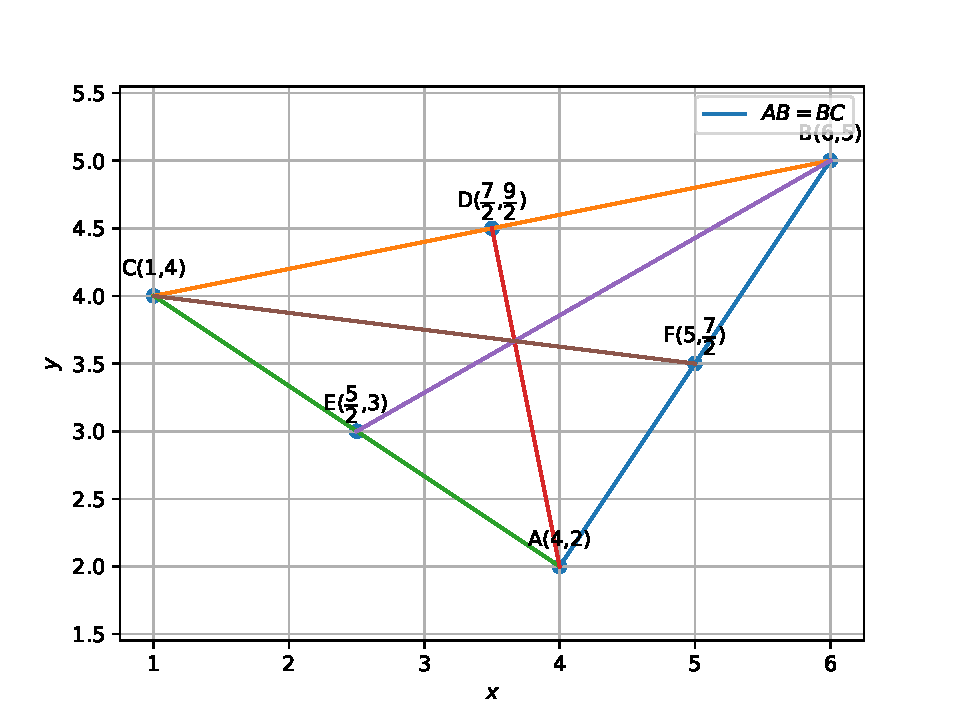
\includegraphics[width=\columnwidth]{chapters/10/7/4/7/figs/dj.pdf}
\caption{}
  \label{fig:chapters/10/7/4/7/Figure}
\end{figure}



\item $ABCD$ is a rectangle formed by the points $\vec{A}(–1, –1), \vec{B}(– 1, 4), \vec{C}(5, 4)$  and  $\vec{D}(5, – 1)$. $\vec{P}, \vec{Q}, \vec{R}$ and $\vec{S}$ are the mid-points of $AB, BC, CD$ and $DA$ respectively. Is the quadrilateral $PQRS$ a square? a rectangle? or a rhombus? Justify your answer.
	\\
	\iffalse
\documentclass[12pt]{article}
\usepackage{graphicx}
%\documentclass[journal,12pt,twocolumn]{IEEEtran}
\usepackage[none]{hyphenat}
\usepackage{graphicx}
\usepackage{listings}
\usepackage[english]{babel}
\usepackage{graphicx}
\usepackage{caption} 
\usepackage{hyperref}
\usepackage{booktabs}
\usepackage{array}
\usepackage{amsmath}   % for having text in math mode
\usepackage{listings}
\lstset{
  frame=single,
  breaklines=true
}
  
%Following 2 lines were added to remove the blank page at the beginning
\usepackage{atbegshi}% http://ctan.org/pkg/atbegshi
\AtBeginDocument{\AtBeginShipoutNext{\AtBeginShipoutDiscard}}
%


%New macro definitions
\newcommand{\mydet}[1]{\ensuremath{\begin{vmatrix}#1\end{vmatrix}}}
\providecommand{\brak}[1]{\ensuremath{\left(#1\right)}}
\providecommand{\norm}[1]{\left\lVert#1\right\rVert}
\newcommand{\solution}{\noindent \textbf{Solution: }}
\newcommand{\myvec}[1]{\ensuremath{\begin{pmatrix}#1\end{pmatrix}}}
\let\vec\mathbf

\begin{document}

\begin{center}
\title{\textbf{Properties of Quadrilaterals}}
\date{\vspace{-5ex}} %Not to print date automatically
\maketitle
\end{center}

\setcounter{page}{1}



\section{10$^{th}$ Maths - Chapter 7}

This is Problem-8 from Exercise 7.4

\begin{enumerate}
\item ABCD is a rectangle formed by the points $\vec{A}(–1, –1), \vec{B}(– 1, 4), \vec{ C}(5, 4) \text{ and } \vec{D}(5, – 1)$. $\vec{P,Q,R} \text{ and } \vec{S}$ are the mid-points of $\vec{AB, BC, CD} \text{ and } \vec{DA}$ respectively. Is the quadrilateral
PQRS a square? a rectangle? or a rhombus? Justify your answer. \\
\fi
\solution 
See Fig. \ref{fig:10/7/4/8Fig3}.
\begin{align}
  \label{eq:10/7/4/8det2f}
  \vec{P} &= \frac{1}{2}\brak{\vec{A}+\vec{B}} =   \frac{1}{2}\brak{\myvec{
  -1 \\
  -1 \\
 } + \myvec{
  -1 \\
  4 \\
 } 
 } = \myvec{
 -1 \\
 \frac{3}{2} \\
 }   \\
 \vec{Q} &= \frac{1}{2}\brak{\vec{B}+\vec{C}} =   \frac{1}{2}\brak{\myvec{
  -1 \\
  4 \\
 } + \myvec{
  5 \\
  4 \\
 } 
 } = \myvec{
 2 \\
 4 \\
 }   \\
 \vec{R} &= \frac{1}{2}\brak{\vec{C}+\vec{D}} =   \frac{1}{2}\brak{\myvec{
  5 \\
  4 \\
 } + \myvec{
  5 \\
  -1\\
 } 
 } = \myvec{
 5 \\
 \frac{3}{2} \\
 }   \\
 \vec{S} &= \frac{1}{2}\brak{\vec{D}+\vec{A}} =   \frac{1}{2}\brak{\myvec{
  5 \\
  -1 \\
 } + \myvec{
  -1 \\
  -1\\
 } 
 } = \myvec{
 2\\
 -1 \\
 }   
\end{align}

\begin{figure}[!h]
	\begin{center}
		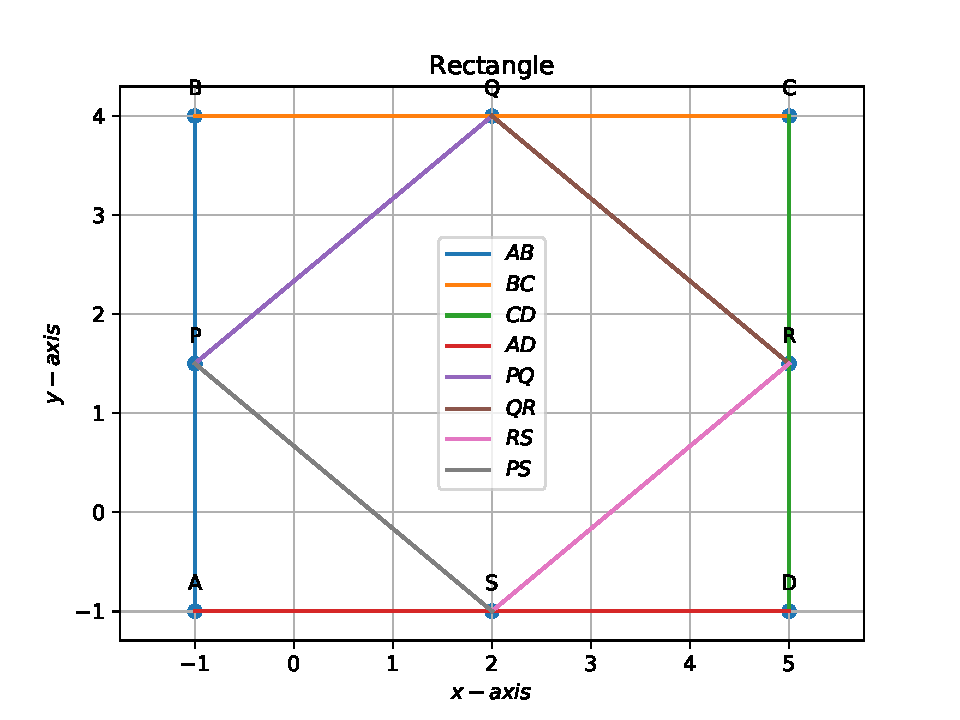
\includegraphics[width=\columnwidth]{chapters/10/7/4/8/figs/problem1.pdf}
	\end{center}
\caption{}
\label{fig:10/7/4/8Fig3}
\end{figure}
We know that PQRS is a parallelogram. To know, if it is a rectangle, we need to ascertain whether any of the two adjacent sides are perpendicular. 
That means $\brak{\vec{Q}-\vec{P}}^\top\brak{\vec{R}-\vec{Q}}$ should be equal to zero. 
\begin{align}
\vec{Q}-\vec{P} &=  \myvec{
 2 \\
 4 \\
 } - \myvec{
 -1 \\
 \frac{3}{2} \\
 } = \myvec{
 3 \\
 \frac{5}{2} \\ 
 } \\
 \vec{R}-\vec{Q} &=  \myvec{
 5 \\
 \frac{3}{2}\\
 } - \myvec{
 2 \\
 4 \\
 } = \myvec{
 3 \\
 -\frac{5}{2} \\ 
 } \\ 
 \brak{\vec{Q}-\vec{P}}^\top\brak{\vec{R}-\vec{Q}} &= \myvec{
 3 & \frac{5}{2}} \myvec{
 3 \\
 -\frac{5}{2} 
 } \neq 0
\end{align}
Therefore PQRS is not a rectangle. Let us check if it is a rhombus. For a rhombus, the diagonals bisect perpendicularly. That means $\brak{\vec{R}-\vec{P}}^\top\brak{\vec{S}-\vec{Q}}$ should be equal to zero. 
\begin{align}
\vec{R}-\vec{P} &=  \myvec{
 5 \\
 \frac{3}{2} \\
 } - \myvec{
 -1 \\
 \frac{3}{2} \\
 } = \myvec{
 6 \\
 0 \\ 
 } \\
 \vec{S}-\vec{Q} &=  \myvec{
 2 \\
 -1 \\
 } - \myvec{
 2 \\
 4 \\
 } = \myvec{
 0 \\
 -5 \\ 
 } \\ 
 \brak{\vec{R}-\vec{P}}^\top\brak{\vec{S}-\vec{Q}} &= \myvec{
 6 & 0} \myvec{
 0 \\
 -5 \\
 } = 0
\end{align}
Therefore $PQRS$ is a rhombus.




\end{enumerate}



